\documentclass[12pt,a4]{article}
%\documentclass{amsart}
\usepackage{amsmath, amsthm}
\usepackage{amssymb}
\usepackage{amsfonts}
\usepackage{array}
\usepackage{graphicx}% use this package if an eps figure is included.
\usepackage{mathrsfs}
\usepackage{multirow}
\usepackage{siunitx}
\usepackage{accents}
\usepackage{enumerate}
\usepackage{accents,color}
\usepackage{cite}

\setlength\topmargin{-1.1in} \addtolength\textheight{2.1in}
\addtolength{\oddsidemargin}{-0.2in}
\addtolength{\evensidemargin}{-0.1in} \textwidth 5.8in
\newcounter{questioncounter}
\newcounter{equestioncounter}
\setlength\parskip{10pt} \setlength\parindent{0in}
\newcommand{\bea}{\begin{eqnarray*}}
\newcommand{\eea}{\end{eqnarray*}}
\newcommand{\beao}{\begin{eqnarray}}
\newcommand{\eeao}{\end{eqnarray}}
\newcommand{\no}{\noindent}

\theoremstyle{plain}
\newtheorem{theorem}{Theorem}[section]
\newtheorem{lemma}[theorem]{Lemma}
\newtheorem{proposition}[theorem]{Proposition}
\newtheorem{corollary}[theorem]{Corollary}
\newtheorem{definition}[theorem]{Definition}
\newtheorem{remark}[theorem]{Remark}


\newcommand{\diam}[0]{\mathrm{diam}}
\newcommand{\rad}[0]{\mathrm{rad}}
\newcommand{\diminf}[0]{\underline{\dim}_B}
\newcommand{\dimsup}[0]{\overline{\dim}_B}
\renewcommand{\Re}[0]{\mathrm{Re}\ }
\renewcommand{\Im}[0]{\mathrm{Im}\ }
\renewcommand{\H}[0]{\mathbb{H}}

%MORE PACKAGES HERE
\newcommand{\R}[0]{\mathbb{R}}
\newcommand{\C}[0]{\mathbb{C}}
\newcommand{\N}[0]{\mathbb{N}}
\newcommand{\Z}[0]{\mathbb{Z}}
\newcommand{\Q}[0]{\mathbb{Q}}
\newcommand{\K}[0]{\mathbb{K}}
\newcommand{\sgn}[0]{\mathrm{sgn}}
\newcommand{\supp}[0]{\mathrm{supp}}

\newcommand{\cred}[1]{{\color{red} #1}}
\newcommand{\cb}[1]{{\color{blue}#1}}

\newcommand{\prodesc}[2]{\left\langle #1 , #2 \right\rangle}


\begin{document}
\title{Multiple Orthogonal Polynomials in several variables}


\author{Fernández, Lidia and Villegas-Recio, Juan Antonio\\
\small University of Granada}
\maketitle

\begin{abstract}
\cred{TODO Write the abstract}
\end{abstract}

\section{Introduction}

Multiple Orthogonality is an extension of the standard orthogonality. It consists of Polynomials (defined on the real line in this introduction) that satisfy orthogonality relations with respect to more than one measure. There are also two different types of multiple orthogonality, which will be explained shortly.

First, let's consider $r$ different real measures $\mu_1,\dots,\mu_r$ such that $\Omega_i=\supp(\mu_i)\subseteq\R$ ($i=1,\dots,r$). We will use multi-indexes $\vec n = (n_1, \dots,n_r)\in \N^r$, and denote $n:=|\vec n| = n_1 + \dots + n_r$. These multi-indexes determine the orthogonality relations with each measure. With these preliminaries we will present the first definition.

\begin{definition}[Type II Multiple Orthogonal Polynomials]
    Let $\vec n = (n_1,\dots,n_r)$. A monic polynomial $P_{\vec n}(x)$ is a type II multiple orthogonal polynomial if $\deg(P_{\vec n})\leq n$ and 
    \begin{equation}
        \label{eq:typeII-MOP}
        \int_{\Omega_i} P_{\vec n}(x) x^k d\mu_i(x) = 0, \ \ \ k=0,\dots,n_{i}-1, \ \ i = 1,\dots,r
    \end{equation}
\end{definition}

This means $P_{\vec n}$ is orthogonal to $1,x,x^2,\dots,n^{n_i-1}$ with respect to each measure $\mu_i$, ($i=1,\dots,r$). If we define the product $\prodesc{f}{g}_i=\int_{\Omega_i}f(x)g(x)d\mu(x)$, conditions \eqref{eq:typeII-MOP} can also be written as
\begin{equation}
    \label{eq:typeII-MOP-dot}
    \prodesc{P_{\vec n}}{x^k}_i = 0, \ \ \ k=0,\dots,n_{i}-1, \ \ i = 1,\dots,r
\end{equation}

There is another type of multiple orthogonality: The type I MOP.

\begin{definition}[Type I Multiple Orthogonal Polynomials]
    \label{def:typeI-univar}
    Let $\vec n = (n_1,\dots,n_r)$. Type I Multiple Orthogonal Polynomials are presented in a vector $(A_{\vec n, 1}(x), \dots, A_{\vec n, r}(x))$, where $\deg(A_{\vec n, i})\leq n_i-1$, ($i=1,\dots,r$) and these polynomials satisfy the relation
    \begin{equation}
        \label{eq:typeI-MOP}
        \sum_{i=1}^r \int_{\Omega_i}A_{\vec n, i}(x) x^k d\mu_i(x) = 0,  \ \ \ k=0,\dots,n-2
    \end{equation}
    and the normalization condition
    \begin{equation}
        \label{eq:typeI-MOP-normalization}
        \sum_{i=1}^r \int_{\Omega_i}A_{\vec n, i}(x) x^{n-1} d\mu_i(x) = 1.
    \end{equation}
    
\end{definition}

As we did previously with the type II MOP, the relations \eqref{eq:typeI-MOP} and \eqref{eq:typeI-MOP-normalization} can be written, using the dot products, as
\begin{equation}
    \sum_{i=1}^r \prodesc{A_{\vec n,i}}{x^k}_i = \left\{\begin{array}{ccl}
        0 &   \text{ if } & k=0,\dots,n-2 \\
        1 & \text{ if } & k=n-1      
    \end{array}\right.
\end{equation}

Whenever the measures are all absolutely continuous with respect to a common positive measure $\mu$ defined in $\Omega = \displaystyle\bigcup_{i=1}^r \Omega_i$, i.e., $d\mu_i = w_i(x) d\mu(x)$, ($i=1,\dots,r$), it is possible to define the \textit{Type I function} as
\begin{equation}
    \label{eq:typeI-function}
    Q_{\vec n}(x)=\sum_{i=1}^r A_{\vec n,i}(x)w_i(x).
\end{equation}
Using the type I function, we can rewrite the orthogonality relations
\begin{equation}
    \label{eq:typeI-MOP-dot}
    \int_\Omega Q_{\vec n}(x) x^k d\mu(x) = \left\{\begin{array}{ccl}
        0 &   \text{ if } & k=0,\dots,n-2 \\
        1 & \text{ if } & k=n-1      
    \end{array}\right.
\end{equation}

Nevertheless, not every multi-index $\vec n\in\N^r$ provides a type I vector of polynomials or a type II polynomial. Let $\vec n = (n_1,\dots,n_r)$ be a multi-index and let $\mu_1,\dots,\mu_r$ be $r$ positive measures. If $(A_{\vec n, 1}(x), \dots, A_{\vec n, r}(x))$ is the vector of type I MOP, then, if we denote
\begin{equation}
    \begin{split}
        A_{\vec n,1}(x) &= a_{n_1-1,1}x^{n_1-1} + a_{n_1-2,1}x^{n_1-2} + \cdots + a_{1,1}x + a_{0,1} \\
        \vdots & \\
        A_{\vec n,r}(x) &= a_{n_r-1,r}x^{n_r-1} + a_{n_r-2,r}x^{n_r-2} + \cdots + a_{1,r}x + a_{0,r}
    \end{split}
\end{equation}
and apply the orthogonality conditions \eqref{eq:typeI-MOP} and \eqref{eq:typeI-MOP-normalization}, then we get a linear system of $n$ equations and $n$ unknown coefficients. Thus, the type I MOP will exist if and only if the following matrix is regular:

\begin{equation}
    \label{eq:MOP-matrix}
    A=\left(\begin{array}{c}
    M_{n_1}^{(1)} \\ \hline
    M_{n_2}^{(2)} \\ \hline
    \vdots \\ \hline
    M_{n_r}^{(r)} \\ 
\end{array}\right), \text{ \ \  where \ \ } M_{n_j}^{(j)} = \begin{pmatrix}
    m_0^{(j)} & m_1^{(j)} & \cdots & m_{n-1}^{(j)} \\
    m_1^{(j)} & m_2^{(j)} & \cdots & m_{n}^{(j)} \\
    \vdots & \vdots & \ddots & \vdots \\
    m_{n_j-1}^{(j)} & m_{n_j}^{(j)} & \cdots & m_{n+n_j-2}^{(j)} \\
\end{pmatrix},
\end{equation}
$j=1,\dots,r$ and $m_k^{(j)}=\displaystyle\int_{\Omega_j} x^k d\mu_j(x)$ are the moments of the measures $(k\geq 0)$.

On the other hand, if we consider the type II polynomial as:
$$
P_{\vec n} = x^n + a_{n-1} x^{n-1} + \cdots + a_1 x + a0
$$
and apply the conditions \eqref{eq:typeII-MOP}, we get another linear system with $n$ equations and $n$ unknown coefficients. In fact, the coefficients matrix of this linear system is $A^t$, the transpose matrix of the type I MOP. Thus, we have the following result.

\begin{proposition}
    \label{prop:existence-of-MOP}
    Given a multi-index $\vec n\in\N^r$ and $r$ positive measures, $\mu_1,\dots,\mu_r$, the following statements are equivalent:
    \begin{enumerate}
        \item There exist an unique vector $(A_{\vec n,1}, \dots, A_{\vec n,r})$ of type I MOP.
        \item There exist an unique type II multiple orthogonal polynomial $P_{\vec n}$.
        \item The matrix $A$ defined in \eqref{eq:MOP-matrix} is regular.
    \end{enumerate}
\end{proposition}

Following this proposition, we provide a new definition.

\begin{definition}
    A multi-index $\vec n = (n_1,\dots,n_r)\in\N^r$ is \textbf{normal} if it satisfies the conditions of the proposition \ref{prop:existence-of-MOP}.
    A system of $r$ measures $\mu_1,\dots,\mu_r$ is \textbf{perfect} if every $\vec n\in\N^r$ is normal.
\end{definition}

There are some perfect systems, standing out the Angelesco systems and the AT-systems, see \cite[Sections 23.1.1 and 23.1.2]{Ismail}

We will be mainly focused on the type II multiple orthogonal polynomials. In the next sections, a definition of type II multiple orthogonal polynomials on several variables will be provided, and also some easy examples and a generalized version of the Jacobi-Piñeiro polynomials. 

\section{Orthogonal Polynomials Systems in several variables}

First of all, we will introduce the notation that will be used. Let $\Pi^d=\R[x_1,\dots,x_d]$ be the space of polynomials in $d$ variables. If $d=2$, we will use the variables $x,y$. For $n\in\N_0$, the space generated by all the degree $n$ monomials is denoted by 
$$
\mathcal{P}_n^d = \left\langle x_1^{k_1} x_2^{k_2} \cdots x_d^{k_d}: k_1+k_2+\cdots +k_d = n, k_1,k_2,\dots,k_d\in\N_0\right\rangle
$$
It is possible to check by induction that the number of different monomials of degree $n$ with $d$ variables is $\displaystyle\binom{n+d-1}{n}$. So, this means
$$
\dim \mathcal{P}_n^d = \binom{n+d-1}{n}.
$$

In order to work with multivariate polynomials, we will use the notation $\mathbb P_n$ as a column polynomial vector. In order to understand this notation, we denote the vector of degree $j$ monomials as
$$
\mathbb{X}_j = \left(x_1^{k_1} x_2^{k_2} \cdots x_d^{k_d}\right)_{k_1+k_2+\cdots +k_d = j}.
$$
For example, if $d=2$ and we use the ``degree reverse lexicographic ordering'' in $\N^2$, then
$$
\mathbb{X}_0=\left(1\right), \mathbb{X}_1=\begin{pmatrix}
    x \\ y
\end{pmatrix}, \mathbb{X}_2=\begin{pmatrix}
    x^2 \\ xy \\ y^2
\end{pmatrix}, \dots, \mathbb{X}_j=\begin{pmatrix}
    x^j \\ x^{j-1}y \\ \vdots \\ y^j
\end{pmatrix}.
$$
Thus, a column polynomial vector of degree $n$ can be represented as
$$
\mathbb{P}_n = G_{n,n}\mathbb{X}_n + G_{n,n-1}\mathbb{X}_{n-1}+\cdots G_{n,1}\mathbb{X}_1 + G_{n,0}\mathbb X_0,
$$
where $G_{n,j}$ are matrices of size $\binom{n+d-1}{n}\times\binom{j+d-1}{j}$ and they are the polynomial's ``coefficients''. Hence, $\mathbb P_n$ is a vector of polynomials whose size is $\binom{n+d-1}{n}$. We will denote 
$$
r_n^d = \dim \mathcal{P}_n^d = \binom{n+d-1}{n}.
$$

Given a multi-dimensional measure $\mu(x_1,\dots,x_d)$, whose support is $\Omega\subseteq\R^d$, we can extend the definition of a multivariate product $\prodesc{f}{g}_\mu$ and its functional $\mathcal{L}_\mu[f\cdot g]$ to column vectors. If $F=(f_1,f_2,\dots,f_n)^t$ and $G=(g_1,g_2,\dots, g_m)^t$ are column vectors of functions of size $n$ and $m$, respectively, then we define
\begin{equation}
    \label{eq:prodesc-matrix}
    \prodesc{F}{G}:=\mathcal{L}_\mu[F\cdot G^T] = \int_\Omega F\cdot G^T d\mu(x_1,\dots,x_d) = \left(\int_\Omega f_i\cdot g_j d\mu(x_1,\dots,x_d)\right)_{i=1,\dots,n;\ \ j = 1,\dots, m}.
\end{equation}

In fact, we are applying the standard product $\prodesc{f_i}{g_j}_\mu$ or the functional $\mathcal L_\mu[f_i\cdot g_j]$ to each pair $i,j$ and placing the results in a matrix.

Let's consider it is possible to build a system of polynomials $\{\mathbb{P}_n\}_{n\geq 0}$ where
$$
\prodesc{\mathbb P_n}{\mathbb P_k}_\mu = \mathcal{L}_\mu[\mathbb P_n \mathbb P_k^t]= \left\{\begin{array}{ccl}
    0_{r_n^d\times r_k^d} &   \text{ if } & k=0,\dots,n-1 \\
    S_n & \text{ if } & k=n      
\end{array}\right. 
$$
Where $S_n$ is a regular squared matrix of size $r_n^d\times r_n^d$.
Due to orthogonality, it is possible to give a equivalent condition:
\begin{equation}
    \label{eq:prodesc-matrix-PX}
    \prodesc{\mathbb P_n}{\mathbb X_k}_\mu = \mathcal{L}_\mu[\mathbb P_n \mathbb X_k^t]= \left\{\begin{array}{ccl}
        0_{r_n^d\times r_k^d} &   \text{ if } & k=0,\dots,n-1 \\
        S_n & \text{ if } & k=n      
    \end{array}\right. 
\end{equation}
Then, $\{\mathbb{P}_n\}_{n\geq 0}$ is called a system of orthogonal polynomials with respect to the measure $\mu$ or the functional $\mathcal L_\mu$. You can check more information about the existence and uniqueness of this system in \cite[Ch. III, Section 3.2]{dunkl_xu_2014}.

\section{Type II MOP in several variables}

In order to respect the original Type II MOP in one variable, given $r\in\N$, $\vec n = (n_1,\dots, n_r)\in\N^r$, $r$ $d$-dimensional measures $\mu_1, \dots, \mu_r$ and their respective dot products defined in \eqref{eq:prodesc-matrix}, we are going to define the type II multiple orthogonality as a monic polynomial vector $\mathbb P_n = \mathbb X_n + \displaystyle\sum_{k=0}^{n-1}G_{n,k} \mathbb X_k$ which satisfies
\begin{equation}
    \label{eq:typeII-MOP-d-variables}
    \prodesc{\mathbb P_n}{\mathbb X_k}_i = 0, \ \ \ k=0,\dots,n_i-1, \ \ \ i=1,\dots,r
\end{equation}
You can check the similarity between conditions \eqref{eq:typeII-MOP-dot} and \eqref{eq:typeII-MOP-d-variables}. Nevertheless, when we work with one variable, it is known the type II polynomial is a monic polynomial whose degree is exactly $|\vec n|$. That is because the number of coefficients of a degree $|\vec n|$ univariate monic polynomial ($|\vec n|$) is equal to the number of orthogonality conditions and the size of matrices $A$ defined in \eqref{eq:MOP-matrix}. Due to the differences between the univariate and the multivariate case, the degree $n$ of the polynomial vector $\mathbb P_n$ might not be equal to $|\vec n|$. For now, this degree $n$ will be considered as unknown, getting to know it later.

As mencioned previously, in the univariate multiple orthogonality, $\deg(P_{\vec n})=|\vec n|$. The main reason this happens is because the condition $\prodesc{P_{\vec n}}{x^k}=0$ is a linear equation (only one). Hence, we are looking for a polynomial with $|\vec n|$ unknown coefficients and we have $|\vec n|$ linear equations deducted from the conditions \eqref{eq:typeII-MOP-dot}. Then, it is possible to build a system of linear equations whose coefficient matrix is $A^t$ given in \eqref{eq:MOP-matrix}.

If we work with $d$ variables, attending to \eqref{eq:prodesc-matrix-PX}, remember the result of $\prodesc{\mathbb P_n}{\mathbb X_k}$ is a matrix of size $r_n^d\times r_k^d$. Thus, it is possible to get $r_n^d\times r_k^d$ linear equations from each orthogonality condition.  

Now, the question is: How many linear equations is it possible to get from a multi-index $\vec n =(n_1, \dots, n_r)$? The answer to this problem is easy since, if we fix $i\in\{1,\dots,r\}$:
\begin{itemize}
    \item $\prodesc{\mathbb P_n}{\mathbb X_0}_i = 0_{r^d_n\times r^d_0}$, we get $r^d_n\times r^d_0$ equations.
    \item $\prodesc{\mathbb P_n}{\mathbb X_1}_i = 0_{r^d_n\times r^d_1}$, we get $r^d_n\times r^d_1$ equations.
    \item \dots
    \item $\prodesc{\mathbb P_n}{\mathbb X_{n_i-1}}_i = 0_{r^d_n\times r^d_{n_i-1}}$, we get $r^d_n\times r^d_{n_i-1}$ equations.
\end{itemize} 
If we collect all the equations, we obtain $r_n^d\cdot\displaystyle\sum_{k=0}^{n_i-1}r^d_k$ linear equations for each $i\in\{1,\dots,r\}$. Collecting the number of equations of each $i$, we finally get the number of equations is 
\begin{equation}
    \label{eq:number-eqs}
    r_n^d \sum_{i=1}^r \sum_{k=0}^{n_i-1} r_k^d.
\end{equation}

On the other hand, since $\mathbb P_n = \mathbb X_n + \displaystyle\sum_{k=0}^{n-1}G_{n,k} \mathbb X_k$, where $G_{n,k}$ are matrices whose dimensions are $r^d_n\times r^d_k$, if we consider $\mathbb P_n$ a vector of degree $n$ monic polynomials, then this matrices give us $\displaystyle\sum_{k=0}^{n-1}r^d_n r^d_k=r^d_n\displaystyle\sum_{k=0}^{n-1} r^d_k$ unknown coefficients.

If we want this system to have only one solution for a multi-index $\vec n$. Then, $\vec n$ is a valid multi-index if there exist a number $n\in\N\cup\{0\}$ such that:
\begin{equation}
    \label{eq:condition-type-ii-general}
    \displaystyle\sum_{k=0}^{n-1} r^d_k = \sum_{i=1}^r \sum_{k=0}^{n_i-1} r_k^d.
\end{equation}

\section{The bidimensional case}

Since this moment, we will assume $d=2$ and $x:=x_1, y:=x_2$. Notice that, in the bidimensional case, $r^2_n = \binom{n+1}{n} = n+1$, which makes things much easier: $\mathbb X_j$ is a polynomial vector of size $j+1$, $\mathbb P_n$ is a vector of size $n+1$, and $G_{n,k}$ is a $(n+1)\times(k+1)$ matrix. Also, the condition \eqref{eq:condition-type-ii-general} gets simpler because some sums become sums of an arithmetic progression. When $d=2$, a multi-index $\vec n =(n_1,\dots,n_r)$ is valid if there exists a number $n\in\N\cup \{0\}$ such that
\begin{equation}
    \label{eq:condition-type-ii}
    n(n+1)=\sum_{i=1}^r n_i (n_i+1).
\end{equation} 

Observe some of the valid multi-indexes and their respective degree $n$.

\begin{table}[h]
    \centering
    \begin{tabular}{|c|c|}
    \hline
    $n$ & Valid multi-indexes when $r=2$ and $d=2$ \\ \hline
    $0$ & $(0,0)$                                  \\ \hline
    $1$ & $(0,1), (1,0)$                           \\ \hline
    $2$ & $(0, 2), (2, 0)$                         \\ \hline
    $3$ & $(0, 3), (2, 2), (3, 0)$                 \\ \hline
    $4$ & $(0, 4), (4, 0)$                         \\ \hline
    $5$ & $(0, 5), (5, 0)$                         \\ \hline
    $6$ & $(0, 6), (3, 5), (5, 3), (6, 0)$         \\ \hline
    $7$ & $(0, 7), (7, 0)$                         \\ \hline
    $8$ & $(0, 8), (5, 6), (6, 5), (8, 0)$         \\ \hline
    $9$ & $(0, 9), (9, 0)$                         \\ \hline
    \end{tabular}
    \caption{Valid multi-indexes when using $r=2$ measures}
    \label{tab:2measuresindexes}
\end{table}

\begin{table}[]
    \centering
    \begin{tabular}{|c|c|}
    \hline
    $n$ & Valid multi-indexes when $r=3$ and $d=2$                                                                                                                                                                           \\ \hline
    $0$ & $(0,0,0)$                                                                                                                                                                                                          \\ \hline
    $1$ & $(0, 0, 1), (0, 1, 0), (1, 0, 0)$                                                                                                                                                                                  \\ \hline
    $2$ & $(0, 0, 2), (0, 2, 0), (1, 1, 1), (2, 0, 0)$                                                                                                                                                                       \\ \hline
    $3$ & $(0, 0, 3), (0, 2, 2), (0, 3, 0), (2, 0, 2), (2, 2, 0), (3, 0, 0)$                                                                                                                                                 \\ \hline
    $4$ & $(0, 0, 4), (0, 4, 0), (1, 2, 3), (1, 3, 2), (2, 1, 3), (2, 3, 1), (3, 1, 2), (3, 2, 1), (4, 0, 0)$                                                                                                                \\ \hline
    $5$ & $(0, 0, 5), (0, 5, 0), (2, 3, 3), (3, 2, 3), (3, 3, 2), (5, 0, 0)$                                                                                                                                                 \\ \hline
    $6$ & \begin{tabular}[c]{@{}c@{}}$(0, 0, 6), (0, 3, 5), (0, 5, 3), (0, 6, 0), (1, 4, 4), (2, 2, 5), (2, 5, 2), (3, 0, 5),$ \\ $(3, 5, 0), (4, 1, 4), (4, 4, 1), (5, 0, 3), (5, 2, 2), (5, 3, 0), (6, 0, 0)$\end{tabular} \\ \hline
    $7$ & \begin{tabular}[c]{@{}c@{}}$(0, 0, 7), (0, 7, 0), (1, 3, 6), (1, 6, 3), (2, 4, 5), (2, 5, 4), (3, 1, 6), (3, 6, 1),$ \\ $(4, 2, 5), (4, 5, 2), (5, 2, 4), (5, 4, 2), (6, 1, 3), (6, 3, 1), (7, 0, 0)$\end{tabular} \\ \hline
    $8$ & \begin{tabular}[c]{@{}c@{}}$(0, 0, 8), (0, 5, 6), (0, 6, 5), (0, 8, 0), (3, 5, 5), (5, 0, 6), (5, 3, 5), (5, 5, 3),$ \\ $(5, 6, 0), (6, 0, 5), (6, 5, 0), (8, 0, 0)$\end{tabular}                                  \\ \hline
    $9$ & \begin{tabular}[c]{@{}c@{}}$(0, 0, 9), (0, 9, 0), (2, 3, 8), (2, 6, 6), (2, 8, 3), (3, 2, 8), (3, 8, 2), (5, 5, 5), (6, 2, 6),$ \\ $(6, 6, 2), (8, 2, 3), (8, 3, 2), (9, 0, 0)$\end{tabular}                       \\ \hline
    \end{tabular}
    \caption{Valid multi-indexes when using $r=3$ measures}
    \label{tab:3measuresindexes}
    \end{table}

    Check this visual representation of the valid multi-indexes when $r=2$ and $r=3$.
    
    \begin{figure}[h]
        \centering\begin{tabular}{cc}
          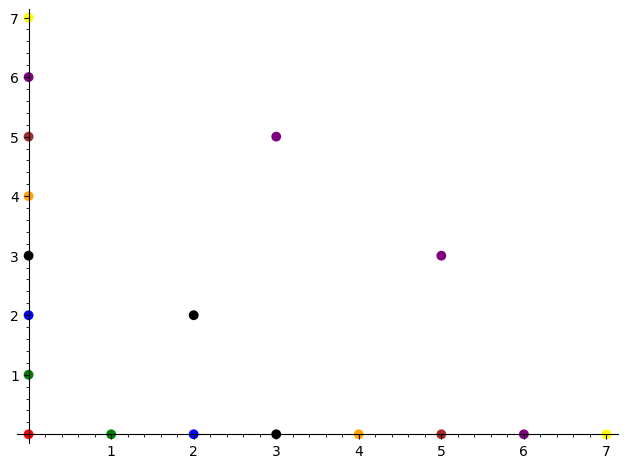
\includegraphics[height=5cm]{./img/puntos2D.png} & 
          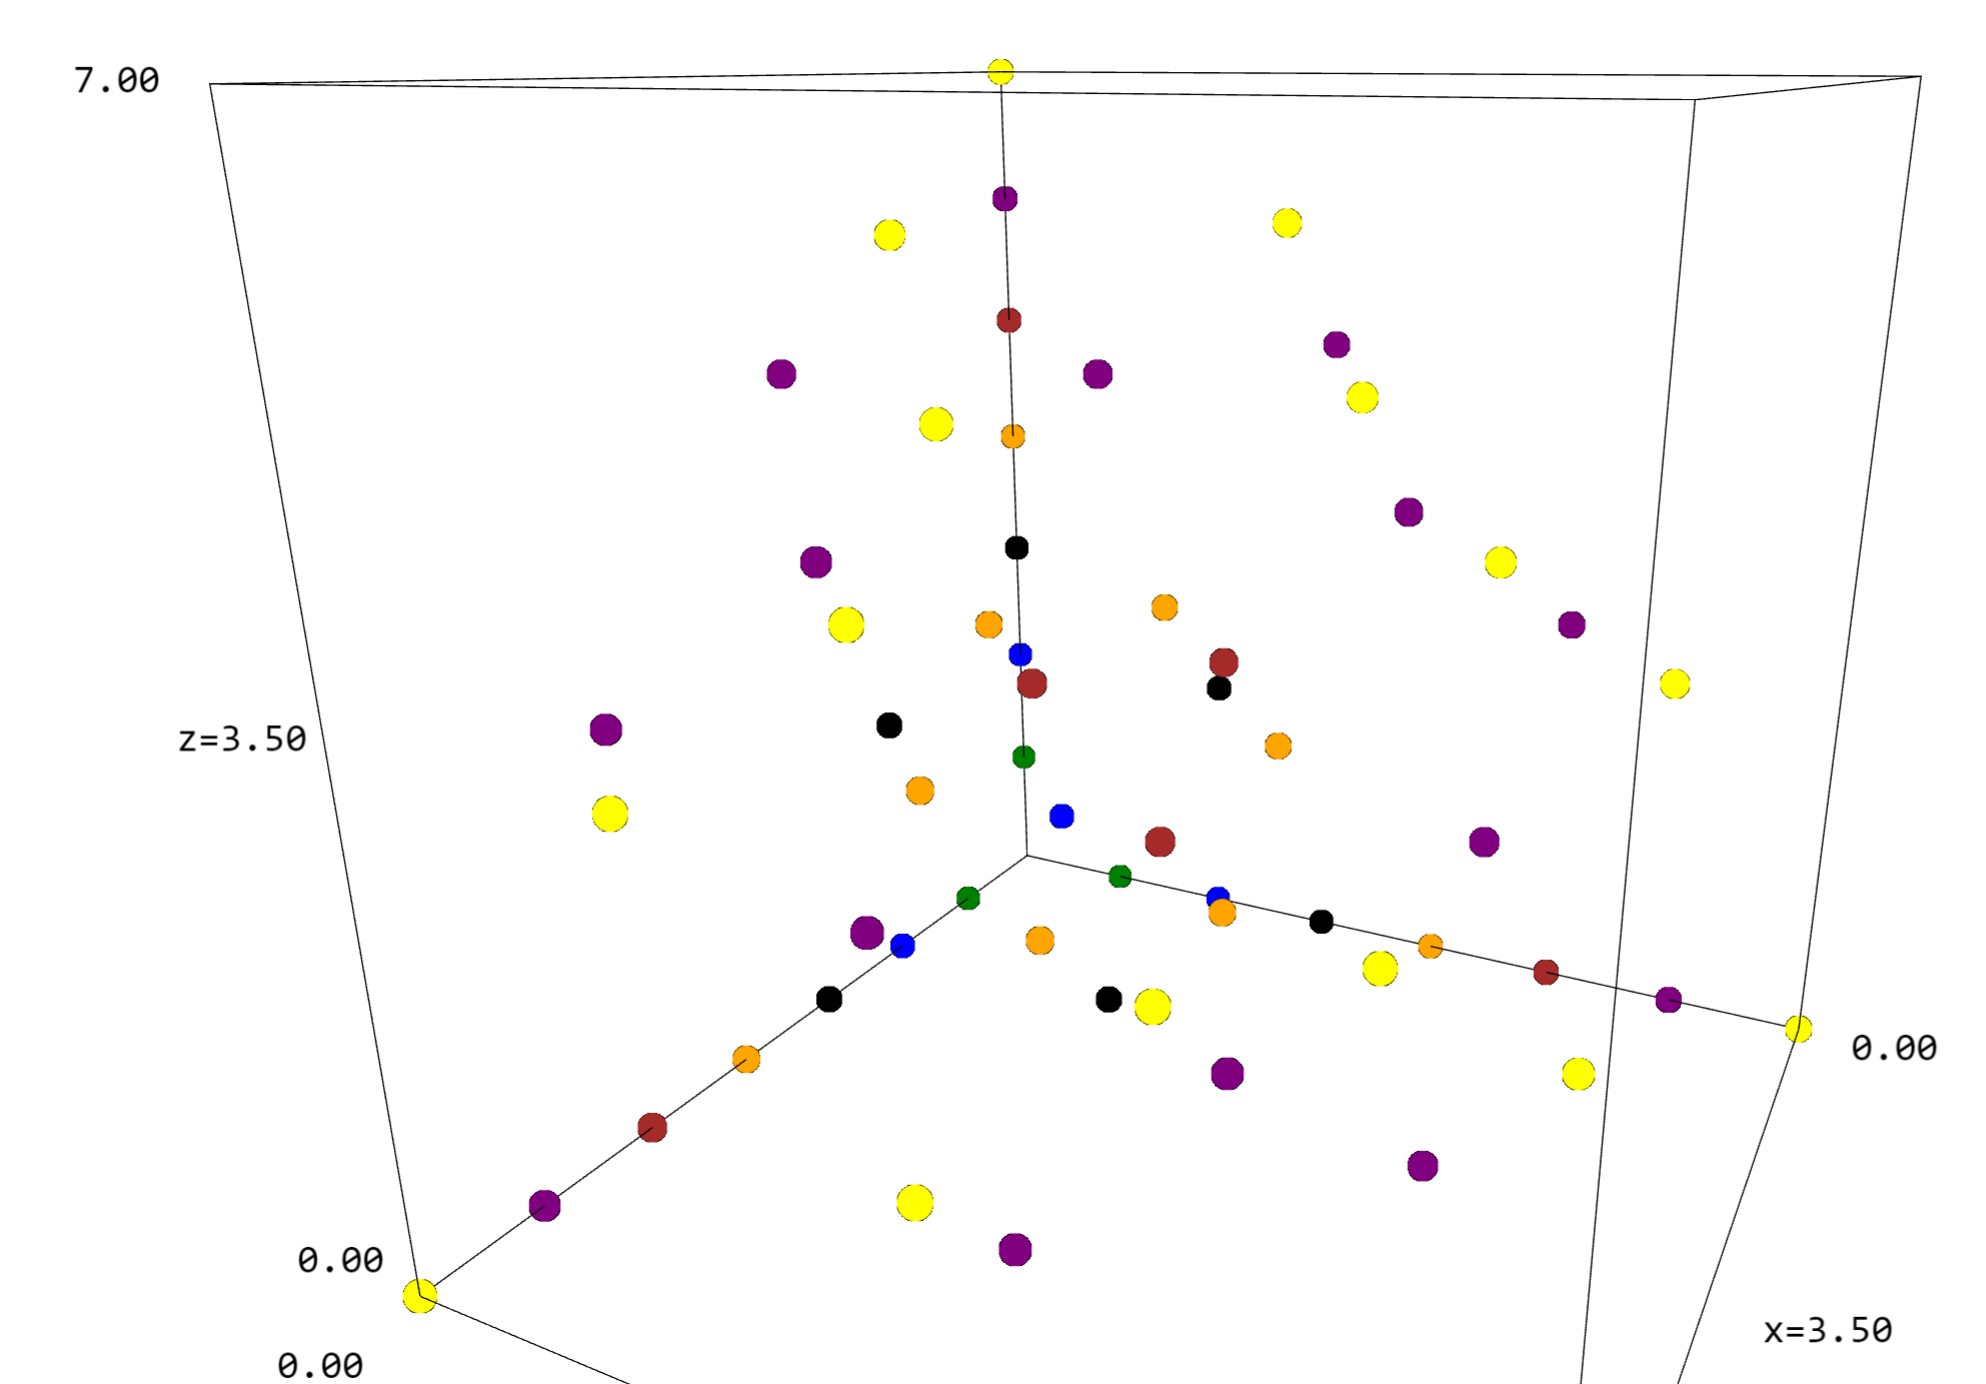
\includegraphics[height=5cm]{./img/puntos3D.png} \\
          (a) $r=2$ & (b) $r=3$  \\
        \end{tabular}
        \caption{Graphic representation of the valid $r$-indexes}
        \label{fig:indexes}
      \end{figure}

\section{Type I MOP in two variables}

Remember the type I multiple orthogonality in definition \ref{def:typeI-univar}. Given $\vec n =(n_1,\dots,n_r)$, it consists of a polynomial vector $(A_{\vec n,1},\dots,A_{\vec n, r})$ where $\deg(A_{\vec n,j})\leq n_j-1$ ($j=1,\dots,r$) and the polynomials satisfy \eqref{eq:typeI-MOP} and \eqref{eq:typeI-MOP-normalization}. This two conditions can be also expresed in a more compact way if we use the dot products, see \eqref{eq:typeI-MOP-dot}.

In order to generalize this type of orthogonality, the first problem is the sum located in the orthogonality condition. This forces us to define polynomials, or polynomial vectors $\mathbb A_{\vec n, j}$, of the same size. If these vectors had different size, it would not be possible to make the sum. This makes impossible to considerate $\mathbb A_{\vec n,j}$ a vector of degree $\leq n_j-1$ polynomials, with size $n_j$. We will tell you how this problem was solved and the definition we give.

Let $\vec n = (n_1,\dots,n_r)\in\N^r$ such that the condition \eqref{eq:condition-type-ii} holds for some $n\in\N$. Then, let $i\in\{1,\dots,n\}$ and, for each $j$, the polynomial $$A_{\vec n, j}^{(i)}(x,y) = g_{n_j-1,n_j-1}^t \mathbb X_{n_j-1} + g_{n_j-1,n_j-2}^t \mathbb X_{n_j-2} + \cdots + g_{n_j-1,0}^t \mathbb X_{0},$$ where $g_{n_j-1,k}\in\R^{k+1}$, ($k=0,\dots,n_j-1$) is a bivariate polynomial such that $\deg A_{\vec n, j}^{(i)} \leq n_j-1$, ($j=1,\dots,r$). Now, given $r$ 2-dimensional measures $\mu_1,\dots,\mu_r$, we will force the polynomials $A_{\vec n, 1}^{(i)}, A_{\vec n, 2}^{(i)}, \dots, A_{\vec n, r}^{(i)}$ to satisfy the first type I multiple orthogonality condition:

\begin{equation}
    \label{eq:first-condition-type-I}
    \sum_{j=1}^r \prodesc{\mathbb X_k}{A_{\vec n,j}^{(i)}}_j = \left\{\begin{array}{ccl}
        0_{(k+1)\times 1} &   \text{ if } & k=0,\dots,n-2 \\
        (e_i)_{n\times 1} = (0,\dots,0,1,0,\dots,0)^t & \text{ if } & k=n-1      
    \end{array}\right.
\end{equation}

You can easily check the number of unknown coefficients of the polynomials $A_{\vec n,j}^{(i)}$ is the same as the number of linear equations given by conditions \eqref{eq:first-condition-type-I}. If we repeat this for every possible $i\in\{1,\dots,n\}$, we get $n$ lists of polynomials $A_{\vec n, j}^{(i)}$, $j=1,\dots,r, i=1,\dots,n$. Now, let's denote
$$
\mathbb A_{\vec n,j} = \begin{pmatrix}
    A_{\vec n, j}^{(1)} \\ \vdots \\ A_{\vec n, j}^{(n)}
\end{pmatrix}_{n\times 1},
$$
a polynomial vector of size $n$ whose components are bivariate polynomials of degree less than or equal to $n_j-1$ ($j=1,\dots,r$) and, fixed $i$, the polynomials $A_{\vec n, 1}^{(i)},\dots,A_{\vec n, r}^{(i)}$ satisfy \eqref{eq:first-condition-type-I}. Thus, the polynomial vectors $\mathbb A_{\vec n,j}$ will satisfy:

\begin{equation}
    \label{eq:condition-type-I}
    \sum_{j=1}^r \prodesc{\mathbb X_k}{\mathbb A_{\vec n,j}}_j = \left\{\begin{array}{ccl}
        0_{(k+1)\times n} &   \text{ if } & k=0,\dots,n-2 \\
        I_n & \text{ if } & k=n-1      
    \end{array}\right.
\end{equation}

Observe the similarity between equations \eqref{eq:typeI-MOP-dot} and \eqref{eq:condition-type-I}.
    
Summarizing, we present the final definitions of the multiple orthogonal polynomials in two variables.

\begin{definition}[Type II MOP in two variables]
    Let $\vec n = (n_1, \dots, n_r)\in \N^r$ such that the condition \eqref{eq:condition-type-ii} holds for certain $n\in\N$. A vector of monic degree $n$ polynomials $\mathbb P_{\vec n}^n = \mathbb X_n + \displaystyle\sum_{k=0}^{n-1} G_{n,k} \mathbb X_k$ is a \textbf{type II Multiple Orthogonal Polynomial Vector} if 
    \begin{equation}
        \label{eq:typeII-MOP-2vars}
        \prodesc{\mathbb X_k}{\mathbb P_{\vec n}^n}_j = 0_{(k+1)\times (n+1)}, \ \ \ k=0,\dots,n_j-1, \ \ \ i=1,\dots,r
    \end{equation}      
\end{definition}

\begin{definition}[Type I MOP in two variables]
    Let $\vec n = (n_1, \dots, n_r)\in \N^r$ such that the condition \eqref{eq:condition-type-ii} holds for certain $n\in\N$. \textbf{Type I Multiple Orthogonal Polynomials Vectors} are presented as $(\mathbb A_{\vec n,1}, \dots, \mathbb A_{\vec n,r})$, where 
    $\mathbb A_{\vec n,j}=(A_{\vec n,j}^{(1)}, \dots, A_{\vec n,j}^{(n)})^t$, $j=1,\dots,r$ and $A_{\vec n,j}^{(i)}$ are polynomials of degree less than or equal to $n_j-1$ for every $i=1,\dots,n$. In addition, these polynomials vectors satisfy the conditions \eqref{eq:condition-type-I}.     
\end{definition}

As the univariate case, from the Type I MOP, in case the 2-dimensional measures are all absolutely continuous with respect to a common positive measure $\mu$ defined in $\Omega = \displaystyle\bigcup_{j=1}^r \Omega_j$, \textit{i.e.}, $d\mu_j = w_j(x,y)d\mu(x,y)$, ($j=1,\dots,r$), we can define the \textit{Type I function}:
\begin{equation}
    \label{eq:type-I-function-2-vars}
    \mathbb Q_{\vec n} = \sum_{j=1}^r \mathbb A_{\vec n,j}w_j(x,y).
\end{equation}
Using this function, it is possible to rewrite \eqref{eq:condition-type-I} as

\begin{equation}
    \prodesc{\mathbb X_k}{\mathbb Q_{\vec n}}_\mu = \left\{\begin{array}{ccl}
        0_{(k+1)\times n} &   \text{ if } & k=0,\dots,n-2 \\
        I_n & \text{ if } & k=n-1 
    \end{array}\right.     
\end{equation}

As we can see, the bivariate case reduces the number of multi-indexes $(n_1,\dots,n_r)$ which it is possible to create multiple orthogonal polynomials with. Whereas in the univariate it is possible to question the existence of MOP for every $\vec n\in \N^r$, in the bivariate case only some of the multi-indexes can give us MOP, those such that there exist $n\in\N$ with $n(n+1)=\displaystyle\sum_{j=1}^r n_j (n_j+1)$. Given a valid $\vec n\in\N^r$, we will say it is \textbf{normal} if it is possible to calculate its type II polynomial $\mathbb P_{\vec n}^n$ and its type I polynomials $\mathbb A_{\vec n,j}$ ($j=1,\dots,r$). The system of 2-dimensional measures $\mu_1,\dots,\mu_r$ will be called \textbf{perfect} if every valid multi-index is normal.

\cb{REVIEW Revisa esto Lidia porque normal y perfecto son conceptos que en una variable tienen sentido porque los tipo I y los tipo II son equivalentes, aquí de momento como poco tan seguros no estamos.}

\cred{TODO Cambiar notación de las primeras definiciones de $P_{\vec n}^n$ y mejorar la explicación de qué es n en este caso.}

\cred{TODO Quitar de la introducción el $n=|\vec n|$ para no confundir con las siguientes secciones}

\section{Biorthogonality}

Let $\mu_1,\dots,\mu_r$ be a perfect system of $r$ 2-dimensional measures. In this section, we will explain an orthogonality relation between the type I and type II MOP. Check the preceding univariate result in \cite[Theorem 23.1.6]{Ismail}.

\begin{theorem}
    \label{th:biorthogonality}
    Given $\vec n, \vec m$, both satisfying \eqref{eq:condition-type-ii} for $n$ and $m$, respectively, the following biorthogonality holds for type I and type II MOP:
    \begin{equation}
        \prodesc{\mathbb P_{\vec n}^n}{\mathbb Q_{\vec m}} = \left\{\begin{array}{ccl}
            0_{(n+1)\times m} &   \text{ if } & \vec m \leq \vec n \\
            0_{(n+1)\times m} &   \text{ if } &  n \leq m -2 \\
            I_{n+1} & \text{ if } & n=m-1 
        \end{array}\right.   
    \end{equation}
\end{theorem}
\begin{proof}
    We will prove each item. First, we have
    \begin{equation*}
        \prodesc{\mathbb P_{\vec n}^n}{\mathbb Q_{\vec m}} = \sum_{j=1}^r \prodesc{\mathbb{P}_{\vec n}^n}{\mathbb A_{\vec m, j}}_j.
    \end{equation*}
    \begin{itemize}
        \item Assume $\vec m \leq \vec n$, this means $m_j \leq n_j \ \ \forall j\in\{1,\dots,r\}$. Then, remember $\mathbb{A}_{\vec m,j}$ is a vector of polynomials of degree less than or equal to $m_j-1 < n_j$ for every $j\in\{1,\dots,r\}$ and $\prodesc{\mathbb P_{\vec n}^n}{\mathbb Q_{\vec m}} =0$ follows from type II orthogonality conditions \eqref{eq:typeII-MOP-2vars}.
        \item  If $n\leq m-2$, then each polynomial of $\mathbb P_{\vec n}^n$ is a linear combination of $\mathbb X_{n-2},\dots,\mathbb X_1,\mathbb X_0$. Then, the type I orthogonality conditions \eqref{eq:condition-type-I} for $0\leq k\leq n-2$ shows $\prodesc{\mathbb P_{\vec n}^n}{\mathbb Q_{\vec m}} =0$.
        \item Finally, if $m=n+1$, then $\mathbb P_{\vec n}^n$ is a vector of degree $m-1$ polynomials. So, $\mathbb P_{\vec n}^n = \mathbb X_{m-1} + \displaystyle\sum_{k=0}^{m-2} G_{k} \mathbb X_{k}$. Because of the previous item, we have
        $$
        \prodesc{\mathbb P_{\vec n}^{m-1}}{\mathbb Q_{\vec m}} = \sum_{j=1}^r \prodesc{\mathbb{P}_{\vec n}^{m-1}}{\mathbb A_{\vec m, j}}_j = \sum_{j=1}^r \prodesc{\mathbb X_{m-1}}{\mathbb A_{\vec m, j}}_j = I_m = I_{n+1},
        $$
        where in the second last equality we have used the normalization condition in \eqref{eq:condition-type-I}.
    \end{itemize}
\end{proof}

Observe the first item emphasises the components of the multi-indexes $\vec n$ and $\vec m$, while the last two items are true for any two multi-indexes with degree $n$ and $m$ whatever their components be.

This result, which is a two-dimensional extension of \cite[Theorem 23.1.6]{Ismail}, will be very useful in order to prove the next result.

\section{Nearest Neighbor Recurrence Relation}

The standard orthogonal polynomials always satisfy a Three-Term Recurrence Relation. That is, given an MOPS $\{P_n\}$ with respect to a dot product $\prodesc{\cdot}{\cdot}$ or its respective functional $\mathcal L$, there exist constants $\alpha_n,\beta_n$ such that
$$
xP_n = P_{n+1}+ \alpha_n P_n + \beta_n P_{n-1}.
$$
The nearest Neighbor Recurrence Relation, in univariate multiple orthogonality, extends this result, allowing us to express a type II polynomial multiplied by $x$: $xP_{\vec n}$ as a linear combination of the polynomial itself, $P_{\vec n}$, a beyond neighbor, \textit{i.e.} $P_{\vec n + e_k}$ and $r$ above neighbors, see \cite[Theorem 23.1.7]{Ismail}. We are going to give a proof of a first generalization to bivariate MOP of this result. 

\begin{theorem} 
    Let $\mu_1,\dots,\mu_r$ be a perfect system of 2-dimensional measures. Let $\vec n\in \N^r$ be a multi-index satisfying \eqref{eq:condition-type-ii} for $n\in\N$ and let us consider a path $\{\overrightarrow{m_k}:k=0,\dots,n+1\}$ where $\overrightarrow{m_0}=\vec 0, \overrightarrow{m_n} = \vec n$, each $\overrightarrow{m_k}$ satisfy \eqref{eq:condition-type-ii} for $k$ and $\overrightarrow{m_k} \leq \overrightarrow{m_{k+1}}$ for $k=0,\dots,n+1$. Then, there exist matrices $A_0,\dots,A_r$ of sizes $(n+1)\times(n-j+1)$,  $(j=0,\dots,r)$ such that
    \begin{equation}
        \label{eq:nearest-neighbor}
        x\mathbb P_{\vec n}^n = L_{{n+1},1} \mathbb P_{\overrightarrow{m_{n+1}}}^{n+1} + A_0 \mathbb P_{\vec n}^n + \sum_{j=1}^r A_j \mathbb P_{\overrightarrow{m_{n-j}}}^{n-j},
    \end{equation}
    where $L_{n+1,1}=(I_{n+1}|0_{(n+1)\times 1})$.

    In addition, $A_j = \prodesc{x\mathbb P_{\vec n}^n}{\mathbb Q_{\overrightarrow{m_{n-j+1}}}}$.
\end{theorem}
\begin{proof}
    As we are in a perfect system, we can assume the existence of $\mathbb P_{\overrightarrow{m_k}}^k$ for every $k=0,\dots,n+1$. As we know, $x\mathbb P_{\vec n}^n$ is a vector of degree $n+1$ polynomials and its size is also $n+1$. It is possible to write  $x\mathbb P_{\vec n}^n$ as a linear combination of $\{\mathbb P_{\overrightarrow{m_k}}^k, k=0,\dots,n+1\}$ whose coefficients are matrices $M_k$:
    $$
    x\mathbb P_{\overrightarrow{n}}^n = \sum_{k=0}^{n+1} M_k \mathbb P_{\overrightarrow{m_k}}^k,
    $$
    where $M_k$ is a $(n+1)\times(k+1)$ matrix ($k=0,\dots,n+1$).

    Observing the leader term of $x\mathbb P_{\overrightarrow{n}}^n$, which is $x\mathbb X_{n}$, and equalizing this to the leader term of $M_{n+1} \mathbb P_{\overrightarrow{m_{n+1}}}^{n+1}$, which is $M_{n+1}\mathbb X_{n+1}$ we can easily check $M_{n+1}=L_{(n+1),1}$. Now, we have
    $$
    \mathbb P_{\overrightarrow{n}}^n = L_{n+1,1}\mathbb P_{\overrightarrow{m_{n+1}}}^{n+1} + \sum_{k=0}^{n} M_k \mathbb P_{\overrightarrow{m_k}}^k.
    $$
    Now, apply the dot product to both sides of the equation by $\mathbb Q_{\overrightarrow{m_l}}$ and observe:
    \begin{itemize}
        \item If $\overrightarrow{m_l}\leq \overrightarrow{m_j}$, which always happens if $l\leq j\leq n+1$, then, due to the first item of theorem \ref{th:biorthogonality}, $\prodesc{\mathbb P_{\overrightarrow{m_j}}^j}{\mathbb Q_{\overrightarrow{m_l}}} = 0_{(j+1)\times l}$ whenever $l\leq j$.
        \item If $j\leq l-2$, then, from the second item of theorem \ref{th:biorthogonality}, $\prodesc{\mathbb P_{\overrightarrow{m_j}}^j}{\mathbb Q_{\overrightarrow{m_l}}} = 0_{(j+1)\times l}.$
        \item Finally, if $j=l-1$, from the last item of theorem \ref{th:biorthogonality} we deduce $\prodesc{\mathbb P_{\overrightarrow{m_j}}^j}{\mathbb Q_{\overrightarrow{m_l}}} = I_{j+1}.$
    \end{itemize}

    Summarizing, we have
    $$
    \prodesc{x\mathbb P_{\vec n}^n}{\mathbb Q_{\overrightarrow{m_l}}} = L_{n+1,1}\prodesc{\mathbb P_{\overrightarrow{m_{n+1}}}^{n+1}}{\mathbb Q_{\overrightarrow{m_l}}} + \sum_{j=0}^n M_j \prodesc{\mathbb P_{\overrightarrow{m_j}}^j}{\mathbb Q_{\overrightarrow{m_l}}}.
    $$
    Applying the previous items deducted from theorem \ref{th:biorthogonality}, we have
    \begin{equation}
        \label{eq:biorthogonality-1}
        \prodesc{x\mathbb P_{\vec n}^n}{\mathbb Q_{\overrightarrow{m_l}}} = M_{l-1} \ \ \ \ l=1,\dots,n+1,
    \end{equation}

    Now, if $l\leq n-r$, then $\overrightarrow{m_l}\leq \overrightarrow{m_{n-r}}$. So, choosing $l\leq n-r$:
    $$
    \prodesc{x\mathbb P_{\vec n}^n}{\mathbb Q_{\overrightarrow{m_l}}} = \sum_{j=1}^r  \prodesc{\mathbb P_{\vec n}^n}{x\mathbb A_{\overrightarrow{m_l},j}}_j.
    $$
    But $x\mathbb A_{\overrightarrow{m_l},j}$ are vectors of degree less than or equal to $(\overrightarrow{m_l})_j\leq (\overrightarrow{m_{n-r}})_j < n_j$. Then, the product vanishes because of type II orthogonality \eqref{eq:typeII-MOP-2vars}. This means
    $$
    \prodesc{x\mathbb P_{\vec n}^n}{\mathbb Q_{\overrightarrow{m_l}}} = M_{l-1} = 0 \ \ \ l = 1, \dots, n-r.
    $$
    Thus, the final expression is
    $$
    \mathbb P_{\overrightarrow{n}}^n = L_{n+1,1}\mathbb P_{\overrightarrow{m_{n+1}}}^{n+1} + \sum_{k=n-r}^{n} M_k \mathbb P_{\overrightarrow{m_k}}^k.
    $$
    If we rename $A_k = M_{n-k}$ for $k=n-r,...,n$, then we get the desired expression \eqref{eq:nearest-neighbor}. 

    Finally, due to \eqref{eq:biorthogonality-1}, $$A_j = M_{n-j} =  \prodesc{x\mathbb P_{\vec n}^n}{\mathbb Q_{\overrightarrow{m_{n-j+1}}}}.$$
\end{proof}
\cb{REVIEW Espero haberlo hecho bien}


\section{Conclusion}
\dots

\nocite{*}
\bibliography{references}{}
\bibliographystyle{plain}


\end{document} 